\documentclass[12pt,letterpaper]{article}
\usepackage{amsmath,amsthm,amsfonts,amssymb,amscd}
\usepackage{listings}
\usepackage{color}
\usepackage{MnSymbol,wasysym}

\definecolor{dkgreen}{rgb}{0,0.6,0}
\definecolor{gray}{rgb}{0.5,0.5,0.5}
\definecolor{mauve}{rgb}{0.58,0,0.82}
\usepackage{biblatex}
\addbibresource{bibliography.bib}
\lstset{%frame=tb,
  language=Bash,
  aboveskip=3mm,
  belowskip=3mm,
  showstringspaces=false,
  columns=flexible,
  basicstyle={\small\ttfamily},
  numbers=none,
  numberstyle=\tiny\color{gray},
  keywordstyle=\color{blue},
  commentstyle=\color{dkgreen},
  stringstyle=\color{mauve},
  breaklines=true,
  breakatwhitespace=true
  tabsize=3
}


\usepackage{hyperref}
\usepackage{graphicx}
\usepackage{enumerate}
\usepackage{fancyhdr}
\usepackage{mathrsfs}
\usepackage[margin=3cm]{geometry}
\setlength{\parindent}{0.0in}
\setlength{\parskip}{0.05in}

% Edit these as appropriate
\newcommand\course{CS432}
\newcommand\semester{Spring 2016}     
\newcommand\hwnum{4}
\newcommand\yourname{Kevin R. Clemmons}
\newcommand\login{oduprogrammer16}

\newenvironment{answer}[1]{
  \subsubsection*{Problem #1}
}

\pagestyle{fancyplain}
\headheight 40pt
\lhead{\yourname\ \\(\login)\\\course\ --- \semester}
\chead{\textbf{\Large Assignment \hwnum}}
\rhead{\today}
\headsep 40pt

\begin{document}

All files mentioned in this file are uploaded into the {\it github} repository.

The \LaTeX code invovled in the generation of this document was aided by the example code provided in the links that Dr. Nelson sent out on January 17, 2016\cite{mohammedaturban2013}. 

This document was compiled on \url{www.sharelatex.com}

\begin{answer}{1}

In order to extract the data located in {\it mln.graphml} a script {\it extractFacebookFriendData.py} was written. Since the given input file was written in xml, the xml-dom parser played a role in extracting the data \cite{pythonsoftwarefoundation2016} . After extracting of the xml-data is complete, an r-script is generated called {\it FacebookPlot.r}. This script generates the graph titled {\it NelsonPlot.pdf} and will display the mean, standard deviation, median,number of friends for Dr. Nelson, number of friends who have more friends than Dr. Nelson and the number of friends who have less friends than Dr. Nelson. 
\newpage 
\begin{figure}[ht!]
\centering
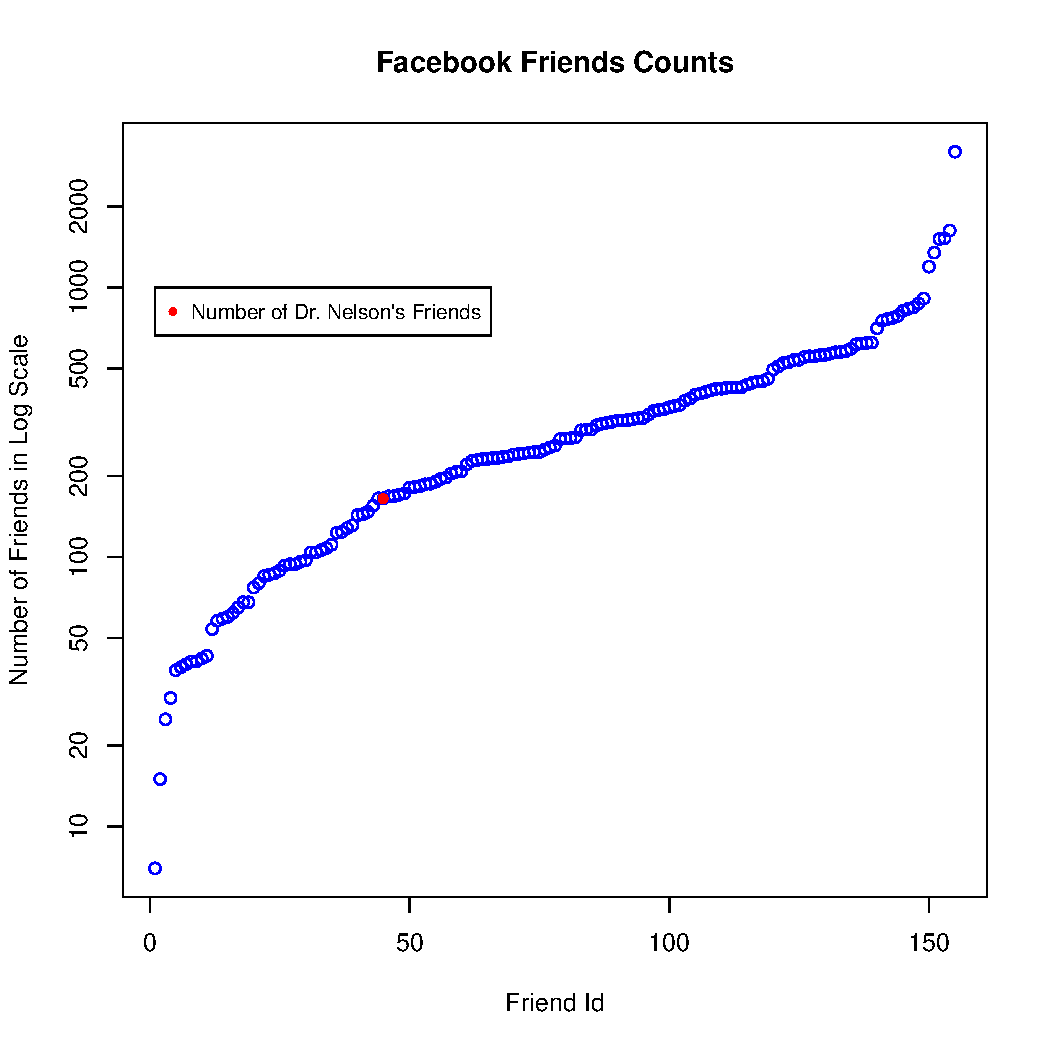
\includegraphics[scale=0.85]{NelsonPlot}
\caption{Number of Friends that Dr. Nelson and His Friends Have}
\label{overflow}
\end{figure}
\newpage
\begin{table}[ht!]
    \centering
    \begin{tabular}{|c|c|}\hline
    \textbf{Measure} & \textbf{Value} \\\hline
     Mean    & 357.73 \\ \hline
     Standard Deviation & 370.70 \\\hline
     Median & 259 \\\hline 
     Number of Friends for Dr. Nelson  & 165 \\\hline
     Number of Friends Who have More Friends than Dr. Nelson & 110 \\\hline Number of Friends Who have Less Friends than Dr. Nelson & 43 \\\hline
    \end{tabular}
    \caption{Statistics from Figure-1, computed by the R-script}
    \label{tab:my_label}
\end{table}
Based on the statistics in Table-1, it is concluded that for Dr. Nelson's facebook account in October 2013, the friendship paradox holds true due to the fact that 110 friends have more friends than Dr. Nelson. 
\newpage
\begin{answer}{2}
In order to extract the followers and the number of their followers a script called {\it twitterFriendData} has been created. The script takes advantage of the Tweepy library to acquire a list of followers and their counts \cite{tweepyFollowerList}. Once the information on the followers and the number of their followers have been obtained, a json file called {\it twitteFollowerCounts.json} will then be generated.

Once the json file is created, another script called {\it createRScript.py} parses the json file and creates an r script called {\it twitterData.r} which produces a graph called {\it KevinTwitterPlot.pdf}. After the graph is generated, script will display the mean, median, standard deviation, number of followers, number of followers who have more followers than KevinClemmons and number of followers who have less followers than KevinClemmons . 
\begin{figure}[ht!]
\centering 
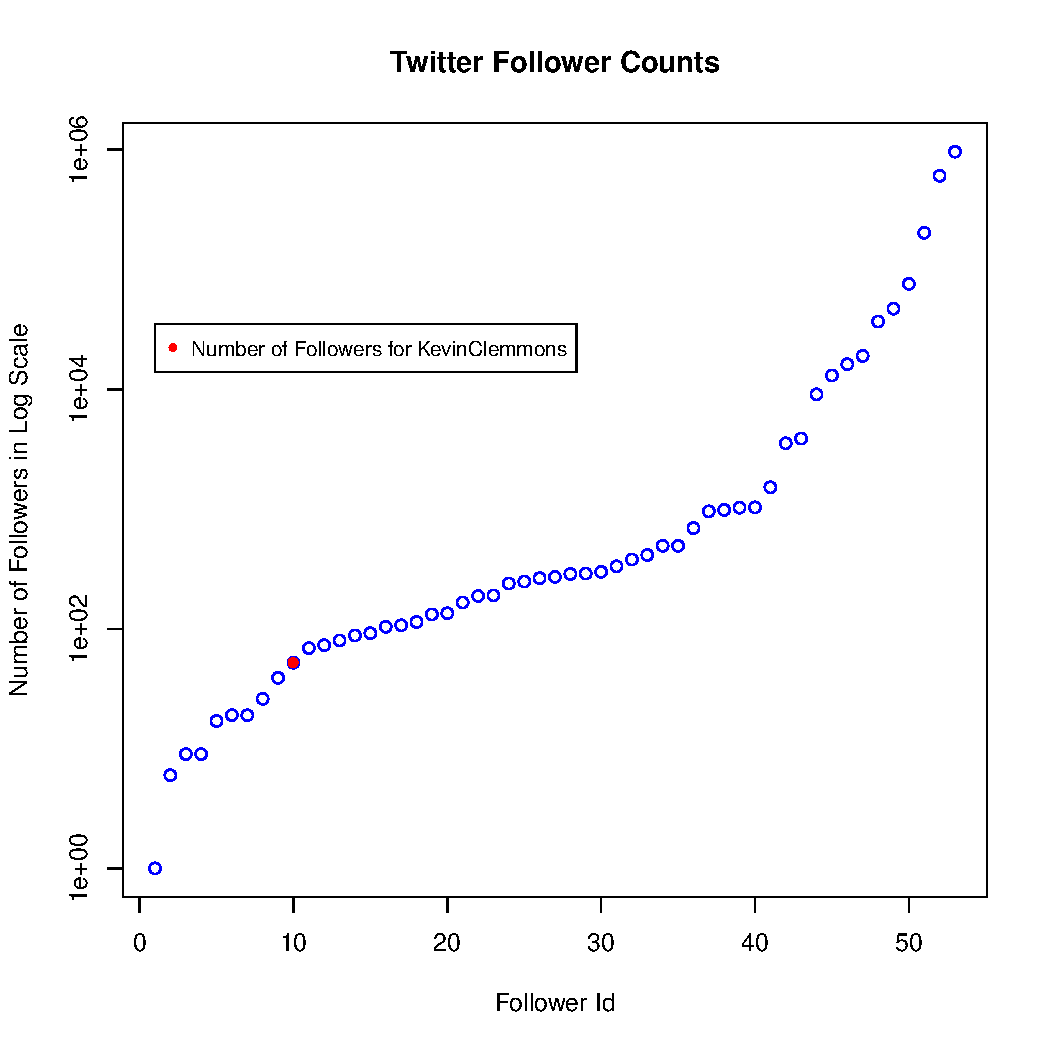
\includegraphics[scale=0.85]{KevinTwitterPlot}
\caption{Number of followers that KevinClemmons and his friends have}
\label{overflow}
\end{figure}
\newpage 

\begin{table}[ht!]
    \centering
    \begin{tabular}{|c|c|}\hline
    \textbf{Measure} & \textbf{Value} \\\hline
     Mean    & 37888.301\\ \hline
     Standard Deviation & 156282.478 \\\hline
     Median & 271 \\\hline 
     Number of Followers for KevinClemmons  & 51 \\\hline
     Number of Followers Who have More Followers than KevinClemmons & 43 \\\hline 
     Number of Followers Who have Less Followers than KevinClemmons & 9 \\\hline
    \end{tabular}
    \caption{Statistics from Figure-2 which computed in the R-script}
    \label{tab:my_label}
\end{table}

Based on the the statistics in Table-2, and the graph in Figure-2, it is concluded that for the twitter account KevinClemmons, the friendship paradox does indeed exist due to the fact that 43 followers have more followers than the account has. \\

{\bf Final Note } \\
Lastly, an interesting thing to note is that the number of Followers who have More Followers than KevinClemmons is equal to the number of friends who have less friends than Dr. Nelson. Perhaps one may want to investigate the possibility of some form of relation exists between the two findings. 
\end{answer}

\newpage
%\bibliographystyle{acm}
\printbibliography

\end{document}
